% ============================================================
% Problemas de Optimización Convexa
% Boyd & Vandenberghe — Capítulo 4
% Presentación Beamer introductoria
% Curso: MM-520 Programación Matemática II
% ============================================================
\documentclass[10pt,aspectratio=169]{beamer}

% --- Paquetes ---
\usepackage[utf8]{inputenc}
\usepackage[T1]{fontenc}
\usepackage[spanish]{babel}
\usepackage{amsmath, amssymb, amsthm, mathtools}
\usepackage{tikz}
\usetikzlibrary{calc,arrows.meta,positioning,shapes.geometric,backgrounds,fit}
\usepackage{graphicx}
\usepackage{booktabs}
\usepackage{xcolor}

% --- Tema y colores ---
\usetheme{Madrid}
\usecolortheme{seahorse}
\definecolor{accentblue}{RGB}{31,73,125}
\definecolor{accentgreen}{RGB}{46,125,50}
\definecolor{accentred}{RGB}{198,40,40}
\setbeamercolor{frametitle}{bg=accentblue,fg=white}
\setbeamercolor{title}{fg=accentblue}
\setbeamertemplate{navigation symbols}{}
\setbeamertemplate{footline}[frame number]

% --- Datos del documento ---
\title{Problemas de Optimización Convexa}
\subtitle{Capítulo 4 --- Boyd \& Vandenberghe}
\author{Optimización Convexa --- MM-520}
\date{\today}

% --- Atajos ---
\newcommand{\R}{\mathbb{R}}
\newcommand{\x}{\mathbf{x}}
\newcommand{\y}{\mathbf{y}}
\newcommand{\z}{\mathbf{z}}
\newcommand{\0}{\mathbf{0}}
\newcommand{\conv}{\operatorname{conv}}
\newcommand{\dom}{\operatorname{dom}}
\newcommand{\epi}{\operatorname{epi}}
\providecommand{\argmin}{\operatorname*{arg\,min}}

% ============================================================
\begin{document}

% ============================================================
\begin{frame}
  \titlepage
\end{frame}

% ------------------------------------------------------------
\section{Esquema del capítulo}
% ------------------------------------------------------------
\begin{frame}{Esquema del capítulo}
  \tableofcontents
\end{frame}

% ============================================================
\section{Problemas de optimización}
% ============================================================
\begin{frame}{Problema de optimización matemática}
  \begin{block}{Forma estándar}
    \[
      \begin{array}{ll}
        \text{minimizar} & f_0(\x) \\
        \text{sujeto a}  & f_i(\x) \le b_i, \quad i=1,\dots,m
      \end{array}
    \]
  \end{block}
  \begin{itemize}
    \item $\x=(x_1,\dots,x_n)\in\R^n$: \emph{variables de optimización} (o de decisión).
    \item $f_0:\R^n\to\R$: \emph{función objetivo} (o de costo).
    \item $f_i:\R^n\to\R$: \emph{funciones de restricción}.
    \item $b_i$: \emph{limite} o \emph{cota} de la restricción $i$.
  \end{itemize}
  \vspace{0.3em}
  \begin{alertblock}{Óptimo}
    El vector $x^\star$ es \emph{óptimo} si tiene el menor valor de $f_0$ entre todos los
    vectores que satisfacen las restricciones.
  \end{alertblock}
\end{frame}

% ------------------------------------------------------------
\begin{frame}{Forma compacta}
  \[
    \begin{array}{ll}
      \text{minimizar} & f_0(\x) \\
      \text{sujeto a}  & f_i(\x) \le 0, \quad i=1,\dots,m \\
                       & h_j(\x)=0, \quad j=1,\dots,p
    \end{array}
  \]
  \begin{itemize}
    \item Restricciones de desigualdad e igualdad se reescalan con la cota.
    \item Solución: $f_0(\x^\star)=\inf\{f_0(\x):f_i(\x)\le 0,\;h_j(\x)=0\}$.
  \end{itemize}
\end{frame}

% ------------------------------------------------------------
\begin{frame}{Óptimo local vs.\ global}
  \begin{columns}
    \column{0.5\textwidth}
      \begin{itemize}
        \item $\x^\star$ \textbf{óptimo local}: $\exists\,R>0$ tal que
          $f_0(\x^\star)\le f_0(\x)$ para todo factible con
          $\|\x-\x^\star\|_2\le R$.
        \item \textbf{Global}: vale para \emph{todo} $\x$ factible.
        \item En general: óptimo global $\Rightarrow$ local, pero no al revés.
        \item La imagen muestra los cuatro casos en una sola función.
      \end{itemize}
    \column{0.5\textwidth}
      \centering
      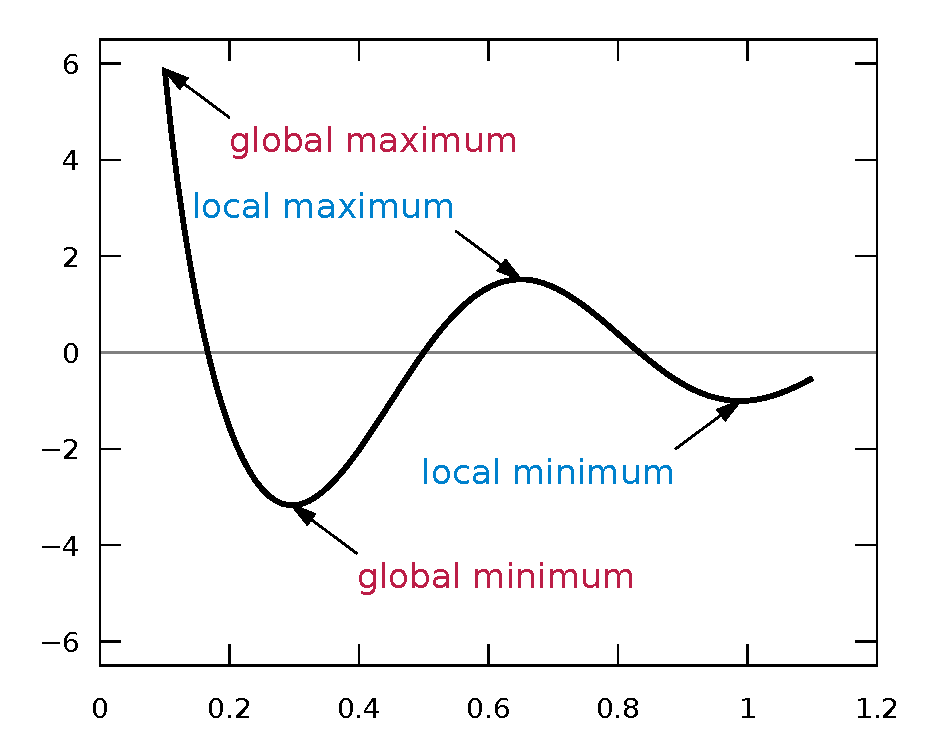
\includegraphics[width=\linewidth]{images/extrema_example_original.pdf}\\[0.3em]
      {\tiny Imagen: KSmrq, Wikimedia Commons, CC BY-SA 3.0.}
  \end{columns}
\end{frame}

% ------------------------------------------------------------
\begin{frame}{Conjunto factible y región de nivel}
  \begin{columns}
    \column{0.5\textwidth}
      \begin{block}{Conjunto factible}
        \[
          \mathcal{D}
          =\bigcap_{i=0}^{m}\dom f_i
          \;\cap\;\bigcap_{j=1}^{p}\dom h_j.
        \]
        Óptimo se busca sobre $\mathcal{D}$.
      \end{block}
    \column{0.5\textwidth}
      \begin{block}{Subnivel}
        Para $t\in\R$:
        \[
          f_0^{-1}((-\infty,t])=\{x\in\dom f_0 : f_0(x)\le t\}.
        \]
        $x^\star$ óptimo global $\Leftrightarrow$
        el subnivel en $f_0(x^\star)$ toca $\mathcal{D}$.
      \end{block}
  \end{columns}
\end{frame}

% ------------------------------------------------------------
\begin{frame}{Tres nociones de solución (y una cuarta)}
  \begin{enumerate}
    \item \textbf{Óptimo global} ($\x^\star$):
      $f_0(\x^\star)\le f_0(\x)$ para todo $\x$ factible.
    \item \textbf{Óptimo local}:
      $\exists\,R>0$ tal que $f_0(\x^\star)\le f_0(\x)$ para todo
      factible con $\|\x-\x^\star\|_2\le R$.
    \item \textbf{Óptimo local ``estricto''}:
      la misma condición con desigualdad estricta, y
      $0<\|\x-\x^\star\|_2\le R$.
  \end{enumerate}
  \vspace{0.4em}
  \begin{block}{$\epsilon$-\'optimo}
    Dado $\epsilon>0$, $\x$ es \textbf{$\epsilon$-\'optimo} si es factible y
    \[
      f_0(\x)\le f_0(\x^\star)+\epsilon.
    \]
    Es una \emph{cuarta noción}: \emph{aproximación práctica} a la
    optimalidad, porque los algoritmos rara vez alcanzan $x^\star$ exacto.
  \end{block}
  \begin{itemize}
    \item Una función estrictamente decreciente sobre un dominio acotado:
      óptimo en un vértice.
    \item Problemas \emph{no convexos} pueden tener óptimos locales no
      globales.
    \item En la práctica basta con $\epsilon$-optimalidad para
      tolerancia numérica.
  \end{itemize}
\end{frame}

% ============================================================
\section{Optimización convexa}
% ============================================================
\begin{frame}{Problema de optimización convexa (POC)}
  \begin{block}{Forma estándar}
    \[
      \begin{array}{ll}
        \text{minimizar} & f_0(\x) \\
        \text{sujeto a}  & f_i(\x)\le 0,\ i=1,\dots,m\\
                         & a_j^\top\x=b_j,\ j=1,\dots,p
      \end{array}
    \]
    con $f_0,f_1,\dots,f_m$ \textbf{convexas}.
  \end{block}
  \begin{itemize}
    \item Restricciones de igualdad \emph{afines} (necesario para convexidad).
    \item $\dom f_i$ son conjuntos convexos (en general: $\R^n$ si $f_i$
      es diferenciable con Hessiano $\succeq 0$).
  \end{itemize}
\end{frame}

% ------------------------------------------------------------
\begin{frame}{El conjunto factible convexo}
  \begin{alertblock}{}
    El conjunto factible de un POC \emph{siempre es convexo}:
    \[
      \mathcal{C}=\{\x\in\R^n: f_i(\x)\le 0,\ a_j^\top\x=b_j\}.
    \]
  \end{alertblock}
  \begin{itemize}
    \item Subniveles de funciones convexas son convexos.
    \item Hiperplanos $\{a^\top\x=b\}$ son convexos.
    \item Intersección de convexos = convexo.
  \end{itemize}
  \vspace{0.4em}
  \begin{flushright}
    \begin{tikzpicture}
      \draw[->] (-0.2,0)--(2.6,0) node[right]{\scriptsize$x_1$};
      \draw[->] (0,-0.2)--(0,2.2) node[above]{\scriptsize$x_2$};
      \begin{scope}
        \clip (0,0) -- (2,0) -- (0,2) -- cycle;
        \fill[accentblue!20] (-1,-1) rectangle (3,3);
      \end{scope}
      \draw[thick,accentblue,->] (0,0) -- (2,0);
      \draw[thick,accentblue,->] (0,0) -- (0,2);
      \draw[thick,accentblue,dashed] (0,0) -- (1,1);
      \node[accentblue] at (1.7,1.5) {\scriptsize$\mathcal{C}$};
    \end{tikzpicture}
  \end{flushright}
\end{frame}

% ------------------------------------------------------------
\begin{frame}{Propiedad clave: óptimo local = global}
  \begin{theorem}[POC]
    Para un problema de optimización convexa, todo óptimo local es
    \emph{óptimo global}.
  \end{theorem}
  \vspace{0.3em}
  \textbf{Esquema de la prueba.}
  Supongamos $x^\star$ local y $\tilde x$ factible con $f_0(\tilde x)<f_0(x^\star)$.
  Para $\theta\in(0,1]$ el punto
  \[
    \x_\theta = x^\star+\theta(\tilde x-x^\star)
  \]
  es factible (convexidad) y
  \[
    f_0(\x_\theta)\le (1-\theta)f_0(x^\star)+\theta f_0(\tilde x)
      < f_0(x^\star).
  \]
  Tomando $\theta\to 0$ contradice la optimalidad local.
  \qed
\end{frame}

% ------------------------------------------------------------
\begin{frame}{Una condición suficiente}
  \begin{block}{Diferenciabilidad}
    Si $f_0$ es diferenciable y convexa, una condición suficiente para
    optimalidad global es:
    \[
      \nabla f_0(\x^\star)^\top(\x-\x^\star)\ge 0\quad
      \forall\,\x\in\mathcal{C}.
    \]
  \end{block}
  \begin{itemize}
    \item Interpretación: ninguna dirección factible decrece $f_0$ en $\x^\star$.
    \item Si $\mathcal{C}=\R^n$, equivale a $\nabla f_0(\x^\star)=0$.
  \end{itemize}
\end{frame}

% ============================================================
\section{Problemas de optimización lineal}
% ============================================================
\begin{frame}{Problema lineal (LP)}
  \begin{block}{Forma estándar}
    \[
      \begin{array}{ll}
        \text{minimizar} & c^\top\x+c_0 \\
        \text{sujeto a}  & G\x\preceq h,\quad A\x=b
      \end{array}
    \]
  \end{block}
  \begin{itemize}
    \item Función objetivo y restricciones son \textbf{afines} (caso particular de convexo).
    \item Conjunto factible = \textbf{poliedro} (intersección de semiespacios e hiperplanos).
    \item Variables en $\R^n$; en algunas variantes $x\succeq 0$.
  \end{itemize}
\end{frame}

% ------------------------------------------------------------
\begin{frame}{Poliedro y poliedro estándar}
  \begin{columns}
    \column{0.5\textwidth}
      \textbf{Poliedro:}
      $\mathcal{P}=\{x:Gx\preceq h,\;Ax=b\}$.
      \begin{itemize}
        \item $G\in\R^{m\times n}$, $A\in\R^{p\times n}$.
        \item $G$ puede ``incluir'' la identidad para imponer cotas.
      \end{itemize}
    \column{0.5\textwidth}
      \textbf{Forma estándar:}
      \begin{align*}
        \text{mín. } & c^\top\x \\
        \text{s.a. }  & A\x=b,\;\x\succeq 0.
      \end{align*}
      \centering
      \begin{tikzpicture}[scale=0.6]
        \draw[->] (-0.2,0)--(2.8,0) node[right]{\scriptsize$x_1$};
        \draw[->] (0,-0.2)--(0,2.2) node[above]{\scriptsize$x_2$};
        \fill[accentblue!20] (0,0) -- (2,0) -- (2,1) -- (0,1) -- cycle;
        \draw[thick,accentblue] (0,0) -- (2,0) -- (2,1) -- (0,1) -- cycle;
        \node[accentblue] at (1,0.6) {\scriptsize$\mathcal{P}$};
      \end{tikzpicture}
  \end{columns}
\end{frame}

% ------------------------------------------------------------
\begin{frame}{Transformaciones equivalentes}
  \begin{itemize}
    \item Restricción de igualdad: $Ax=b$ $\Leftrightarrow$ dos desigualdades $Ax\le b$ y $Ax\ge b$.
    \item Variable libre: $x=x^+-x^-$ con $x^+,x^-\ge 0$.
    \item Minimizar $c^\top\x$ = maximizar $(-c)^\top\x$.
    \item Inequivalencia ``estricta'' $a^\top\x<b$ se puede sustituir por
      $a^\top\x\le b-\epsilon$ con $\epsilon>0$ prefijado.
  \end{itemize}
\end{frame}

% ------------------------------------------------------------
\begin{frame}{Ejemplo: planificación de producción}
  Una fábrica produce 3 productos. Beneficios por unidad: $c=(3,1,2)$.
  Recursos y consumo por unidad:
  \[
    A=\begin{pmatrix}1&2&1\\3&0&2\end{pmatrix},\;
    b=\begin{pmatrix}4\\6\end{pmatrix},\;
    x\ge 0.
  \]
  \begin{align*}
    \text{máx. } & c^\top\x \\
    \text{s.a. }  & A\x\le b,\ \x\ge 0.
  \end{align*}
  Solución en un vértice del poliedro factible.
\end{frame}

% ------------------------------------------------------------
\begin{frame}{Programación lineal-fraccional (LFP)}
  \begin{block}{Forma estándar}
    \[
      \begin{array}{ll}
        \text{minimizar} & \dfrac{c^\top\x + d}{e^\top\x + f} \\[0.6em]
        \text{sujeto a}  & G\x\preceq h,\quad A\x=b
      \end{array}
    \]
    con denominador positivo: $e^\top\x+f>0$ sobre la región factible.
  \end{block}
  \begin{itemize}
    \item \textbf{Objetivo}: cociente de funciones afines (numerador y
      denominador).
    \item Restricciones \textbf{lineales} (afines): el conjunto factible es
      un \emph{poliedro}.
    \item Es un caso intermedio entre LP y convexo general.
  \end{itemize}
\end{frame}

% ------------------------------------------------------------
\begin{frame}{LFP como problema convexo}
  \begin{alertblock}{}
    El problema LFP \emph{siempre} se puede reformular como un LP
    mediante el cambio de variables:
    \[
      y=\frac{\x}{e^\top\x+f},\qquad
      t=\frac{1}{e^\top\x+f},
    \]
    con $t>0$.
  \end{alertblock}
  \begin{itemize}
    \item El problema transformado es lineal en $(y,t)$.
    \item Por tanto LFP es \textbf{resoluble tan eficientemente como un LP}.
    \item Ejemplo clásico: maximizar la razón \emph{retorno / riesgo}
      en optimización de portafolios.
  \end{itemize}
\end{frame}

% ============================================================
\section{Problemas de optimización cuadrática}
% ============================================================
\begin{frame}{Problema cuadrático (QP)}
  \begin{block}{Forma estándar}
    \[
      \begin{array}{ll}
        \text{minimizar} & (1/2)\,\x^\top P\x+q^\top\x+r \\
        \text{sujeto a}  & G\x\preceq h,\quad A\x=b
      \end{array}
    \]
  \end{block}
  \begin{itemize}
    \item $P\in\mathbb{S}_+^n$ \emph{simétrica definida no-negativa} (para convexidad).
    \item Función objetivo es cuadrática estrictamente convexa si $P\succ 0$.
    \item LP = QP con $P=0$.
  \end{itemize}
\end{frame}

% ------------------------------------------------------------
\begin{frame}{Diagrama de QP convexo}
  \centering
  \begin{tikzpicture}[scale=0.85]
    % Region factible (un disco interseccion)
    \begin{scope}
      \clip (0,0) rectangle (6,4);
      \fill[accentblue!15] (0,0) rectangle (6,4);
    \end{scope}
    % Curvas de nivel de la cuadratica
    \foreach \r in {0.5,0.9,1.3,1.7,2.1}{
      \draw[accentred,thick,opacity=0.6] (3,2) circle (\r);
    }
    \node[accentred] at (5.4,2) {\scriptsize$f_0$ nivel};
    % Solución óptima
    \fill[accentgreen] (2.4,1.2) circle (2pt);
    \node[accentgreen,below right] at (2.4,1.2) {\scriptsize$x^\star$};
    \draw[->,thick] (3,2) -- (2.4,1.2);
  \end{tikzpicture}
\end{frame}

% ------------------------------------------------------------
\begin{frame}{Casos particulares y aplicaciones}
  \begin{description}
    \item[QP con restricciones lineales] Límite natural entre LP y convexo general.
    \item[$\ell_2$-regularización (ridge)]
      $\min\ \|Ax-b\|_2^2+\lambda\|x\|_2^2$: caso $P=2(A^\top A+\lambda I)$.
    \item[Control óptimo LQR]
      Estado $x_{t+1}=A_tx_t+B_tu_t$; costo $\sum x_t^\top Qx_t+u_t^\top Ru_t$.
    \item[SVM con kernel cuadrático]
      $\min \|w\|^2$ s.a. restricciones lineales de margen.
  \end{description}
\end{frame}

% ============================================================
\section{Programación geométrica}
% ============================================================
\begin{frame}{Forma posinomial (GP)}
  \begin{block}{}
    Una función $f:\R^n_{++}\to\R$ es \textbf{posinomial} si existe
    $c_k>0$ y $a_{kj}\in\R$ tales que
    \[
      f(\x)=\sum_{k=1}^{K}c_k x_1^{a_{k1}}x_2^{a_{k2}}\cdots x_n^{a_{kn}}.
    \]
  \end{block}
  \begin{itemize}
    \item Cada \emph{monomio} $c_k \x^{\mathbf{a}_k}$ con exponentes reales
      cualesquiera.
    \item Suma de monomios con coeficientes positivos.
  \end{itemize}
\end{frame}

% ------------------------------------------------------------
\begin{frame}{Forma monomial y el problema GP}
  \begin{block}{Monomial}
    $f(\x)=c\,x_1^{a_1}x_2^{a_2}\cdots x_n^{a_n}$ con $c>0$.
  \end{block}
  \begin{block}{Programa geométrico}
    \[
      \begin{array}{ll}
        \text{minimizar} & f_0(\x) \\
        \text{sujeto a}  & f_i(\x)\le 1,\ i=1,\dots,m,\\
                         & h_j(\x)=1,\ j=1,\dots,p
      \end{array}
    \]
    con $f_0,\dots,f_m$ posinomiales y $h_1,\dots,h_p$ monomiales.
  \end{block}
\end{frame}

% ------------------------------------------------------------
\begin{frame}{GP no es convexo --- pero su cambio de variables sí}
  Sustituir $y_i=\log x_i$, $b_{kj}=\log c_k$ y
  $\tilde f(\y)=\log f(\x)$:
  \begin{itemize}
    \item Monomios: $\log(c\,\x^{\mathbf{a}})=\log c + \mathbf{a}^\top\y$ \quad(afín en $\y$).
    \item Posinomiales: $\log\!\left(\sum_k c_k\x^{\mathbf{a}_k}\right)$
      es \textbf{log-sum-exp} --- \emph{convexa}.
  \end{itemize}
  \begin{alertblock}{}
    GP en variable $\x$ \quad $\longleftrightarrow$ \quad
    \textbf{Problema convexo} en variable $\y=\log\x$.
  \end{alertblock}
\end{frame}

% ------------------------------------------------------------
\begin{frame}{Ejemplo clásico: mínimo de posinomio}
  \[
    \min_{x>0}\ x^{-1}y^{-1/2}z^{-1} + 2.3\,x\,y^2z + 5\,x^{1/2}y
  \]
  \[
    \text{s.a. } (1/3)x^{-2}y^{-2} + (4/3)y^{1/2}z^{-1}\le 1,\quad
    x+y\le 1.
  \]
  El cambio $y=\log x$, $y_2=\log y$, $y_3=\log z$ lo convierte en un
  problema convexo resoluble eficientemente.
\end{frame}

% ============================================================
\section{Restricciones con desigualdades generalizadas}
% ============================================================
\begin{frame}{Cono propio y orden parcial}
  \begin{definition}
    Un cono $K\subseteq\R^m$ es \textbf{propio} si:
    \begin{itemize}
      \item $K$ es convexo.
      \item $K$ es cerrado.
      \item $K$ tiene interior no vacío.
      \item $K\cap(-K)=\{0\}$.
    \end{itemize}
  \end{definition}
  \begin{itemize}
    \item $K$ define un orden parcial: $y\preceq_K z$ $\Leftrightarrow$ $z-y\in K$.
    \item Ejemplos: $\R_+^m$ (cono no-negativo), $S_+^m$ (matrices
      semidefinidas positivas).
  \end{itemize}
\end{frame}

% ------------------------------------------------------------
\begin{frame}{POC con desigualdades generalizadas}
  \begin{block}{}
    \[
      \begin{array}{ll}
        \text{minimizar} & f_0(\x) \\
        \text{sujeto a}  & f_i(\x)\preceq_{K_i} 0,\ i=1,\dots,m,\\
                         & h_j(\x)=0
      \end{array}
    \]
  \end{block}
  \begin{itemize}
    \item $f_i:\R^n\to\R^{m_i}$, $K_i\subseteq\R^{m_i}$ cono propio.
    \item Conexión con desigualdades estándar: $K_i=\R_+^{m_i}$ recupera
      $f_i(\x)\le 0$.
  \end{itemize}
\end{frame}

% ------------------------------------------------------------
\begin{frame}{Cono dual y conos importantes}
  \begin{block}{Cono dual}
    $K^\star=\{y:y^\top x\ge 0\ \forall x\in K\}$.
  \end{block}
  \begin{itemize}
    \item $\R_+^m$: dual = $\R_+^m$ (autoduval).
    \item $S_+^m$: dual = $S_+^m$ (autoduval).
    \item Cono de Lorentz (segundo orden):
      $\mathcal{L}_m=\{(x,t):\|x\|_2\le t\}$; dual $\mathcal{L}_m^\star=\mathcal{L}_m$.
  \end{itemize}
\end{frame}

% ------------------------------------------------------------
\begin{frame}{Ejemplo: SDP (programa semidefininido)}
  \begin{block}{}
    \[
      \begin{array}{ll}
        \text{minimizar} & c^\top\x \\
        \text{sujeto a}  & x_1 F_1+\cdots+x_n F_n + G\preceq_{S_+^m} 0\\
                         & A\x=b
      \end{array}
    \]
  \end{block}
  \begin{itemize}
    \item $F_i,G\in S^m$ matrices simétricas.
    \item Es un POC con $K_i=S_+^m$.
    \item Generaliza LP ($S_+^1\cong\R_+$) y muchos QP.
  \end{itemize}
\end{frame}

% ============================================================
\section{Optimización vectorial}
% ============================================================
\begin{frame}{Problema vectorial (VOP)}
  \begin{block}{}
    \[
      \begin{array}{ll}
      \text{minimizar} & (f_1(\x),\dots,f_q(\x)) \\
      \text{sujeto a}  & \x\in\mathcal{C}
      \end{array}
    \]
  \end{block}
  \begin{itemize}
    \item Varios objetivos \textbf{en conflicto} $\Rightarrow$ no hay un único ``mejor''.
    \item La teoría: \emph{óptimo de Pareto} (Pareto-óptimo) --- un vector no dominado.
  \end{itemize}
\end{frame}

% ------------------------------------------------------------
\begin{frame}{Óptimo de Pareto y débilmente Pareto}
  \begin{definition}[Pareto-óptimo]
    $\x^\star\in\mathcal{C}$ es \emph{Pareto-óptimo} si no existe
    $\x\in\mathcal{C}$ con $f_i(\x)\le f_i(\x^\star)$ para todo $i$ y
    alguna desigualdad estricta.
  \end{definition}
  \begin{definition}[Débil]
    $\x^\star$ es \emph{débilmente Pareto} si no existe
    $\x\in\mathcal{C}$ con $f_i(\x)<f_i(\x^\star)$ para todo $i$.
  \end{definition}
\end{frame}

% ------------------------------------------------------------
\begin{frame}{Ponderación escalar (método de pesos)}
  \begin{block}{}
    Fijar $\lambda\succ 0$, $\sum\lambda_i=1$, y resolver
    \[
      \min_{\x\in\mathcal{C}}\ \lambda^\top f(\x)
        =\sum_{i=1}^{q}\lambda_i f_i(\x).
    \]
  \end{block}
  \begin{itemize}
    \item Si $\x^\star_\lambda$ es único $\Rightarrow$ Pareto-óptimo.
    \item Si $\x^\star_\lambda$ es Pareto-óptimo para todo $\lambda\succ 0$
      y el problema es convexo, la curva de trade-off se reconstruye.
    \item No todos los Pareto-óptimos se obtienen con un único $\lambda$.
  \end{itemize}
\end{frame}

% ------------------------------------------------------------
\begin{frame}{Imagen: frente de Pareto}
  \centering
  \begin{tikzpicture}[scale=0.85]
    \draw[->] (0,0)--(6,0) node[right]{\scriptsize$f_1$};
    \draw[->] (0,0)--(0,4.2) node[above]{\scriptsize$f_2$};
    % Region factible
    \begin{scope}
      \clip (0,0) rectangle (6,4);
      \fill[accentblue!12] (0,0) rectangle (6,4);
    \end{scope}
    % Frente de Pareto (curva no decreciente)
    \draw[thick,accentred,domain=0.5:5.2,samples=60]
      plot(\x,{3.5-0.45*sqrt(\x)}) node[above right,accentred]{\scriptsize frente};
    % Puntos
    \foreach \x in {0.6,1.4,2.4,3.6,4.8}{
      \fill[accentgreen] (\x,{3.5-0.45*sqrt(\x)}) circle(1.4pt);
    }
  \end{tikzpicture}
\end{frame}

% ============================================================
\section{Resumen}
% ============================================================
\begin{frame}{Mapa general de problemas convexos}
  \centering
  \begin{tikzpicture}[
    node distance=0.5cm and 0.7cm,
    every node/.style={font=\small},
    box/.style={rectangle,draw,fill=accentblue!8,rounded corners,
                minimum width=3.2cm,minimum height=0.9cm,align=center},
    arrow/.style={-Stealth,thick}
  ]
    \node[box] (lp) {LP\\$\min c^\top x$};
    \node[box,below=of lp] (lfp) {LFP\\$\min \frac{c^\top x+d}{e^\top x+f}$};
    \node[box,below=of lfp] (qp) {QP\\$\min x^\top P x$};
    \node[box,below=of qp] (gp) {GP\\posinomios};
    \node[box,below=of gp] (socp) {SOCP\\$\|A x+b\|\le c^\top x+d$};
    \node[box,below=of socp] (sdp) {SDP\\restricc. matriciales};
    \node[box,right=1.6cm of qp,fill=accentgreen!10] (coc) {POC general};
    \draw[arrow] (lp)--(coc) node[midway,above,sloped]{\scriptsize caso particular};
    \draw[arrow] (lfp)--(coc);
    \draw[arrow] (qp)--(coc);
    \draw[arrow] (gp)--(coc);
    \draw[arrow] (socp)--(coc);
    \draw[arrow] (sdp)--(coc);
  \end{tikzpicture}
\end{frame}

% ------------------------------------------------------------
\begin{frame}{Mensajes para llevar}
  \begin{enumerate}
    \item \textbf{POC} = minimizar convexa, restricciones convexas e iguales afines.
    \item \textbf{Óptimo local = global} (y por tanto, los algoritmos encuentran
      la mejor solución posible).
    \item \textbf{LP, LFP, QP, GP, SOCP, SDP} son casos particulares, todos
      resolubles eficiente y confiablemente.
    \item \textbf{GP} se vuelve convexo con el cambio $y=\log x$.
    \item \textbf{Desigualdades generalizadas} extienden LP $\to$ SDP vía conos propios.
    \item \textbf{Optimización vectorial} se reduce a múltiples escalares (ponderación),
      produciendo el \emph{frente de Pareto}.
  \end{enumerate}
\end{frame}

% ------------------------------------------------------------
\begin{frame}{Referencias}
  \begin{thebibliography}{9}
    \bibitem{BOV} S. Boyd y L. Vandenberghe.
      \emph{Convex Optimization}. Cambridge University Press, 2004.
      \texttt{stanford.edu/~boyd/cvxbook/}
    \bibitem{BVnotes} S. Boyd y L. Vandenberghe.
      \emph{Notes for EE364B --- Convex Optimization II}. Stanford.
    \bibitem{Nem} Yu. Nesterov y A. Nemirovski.
      \emph{Interior-Point Polynomial Algorithms in Convex Programming}. SIAM, 1994.
    \bibitem{BenTal} A. Ben-Tal y A. Nemirovski.
      \emph{Lectures on Modern Convex Optimization}. SIAM, 2001.
  \end{thebibliography}
\end{frame}

\end{document}
